\section{Pre-study}
	\subsection{Solution today}
		\subsubsection{Existing functionality}
Since the application already is considered a working prototype, we will provide a list which gives a description for the functionality. Working functionality is in this report defined as the functionality that is implemented in the frontend or backend. If something is implemented backend it has to be used frontend. A more detailed techincal description is found in the architecture-section.

\begin{figure}[h!]
\begin{center}
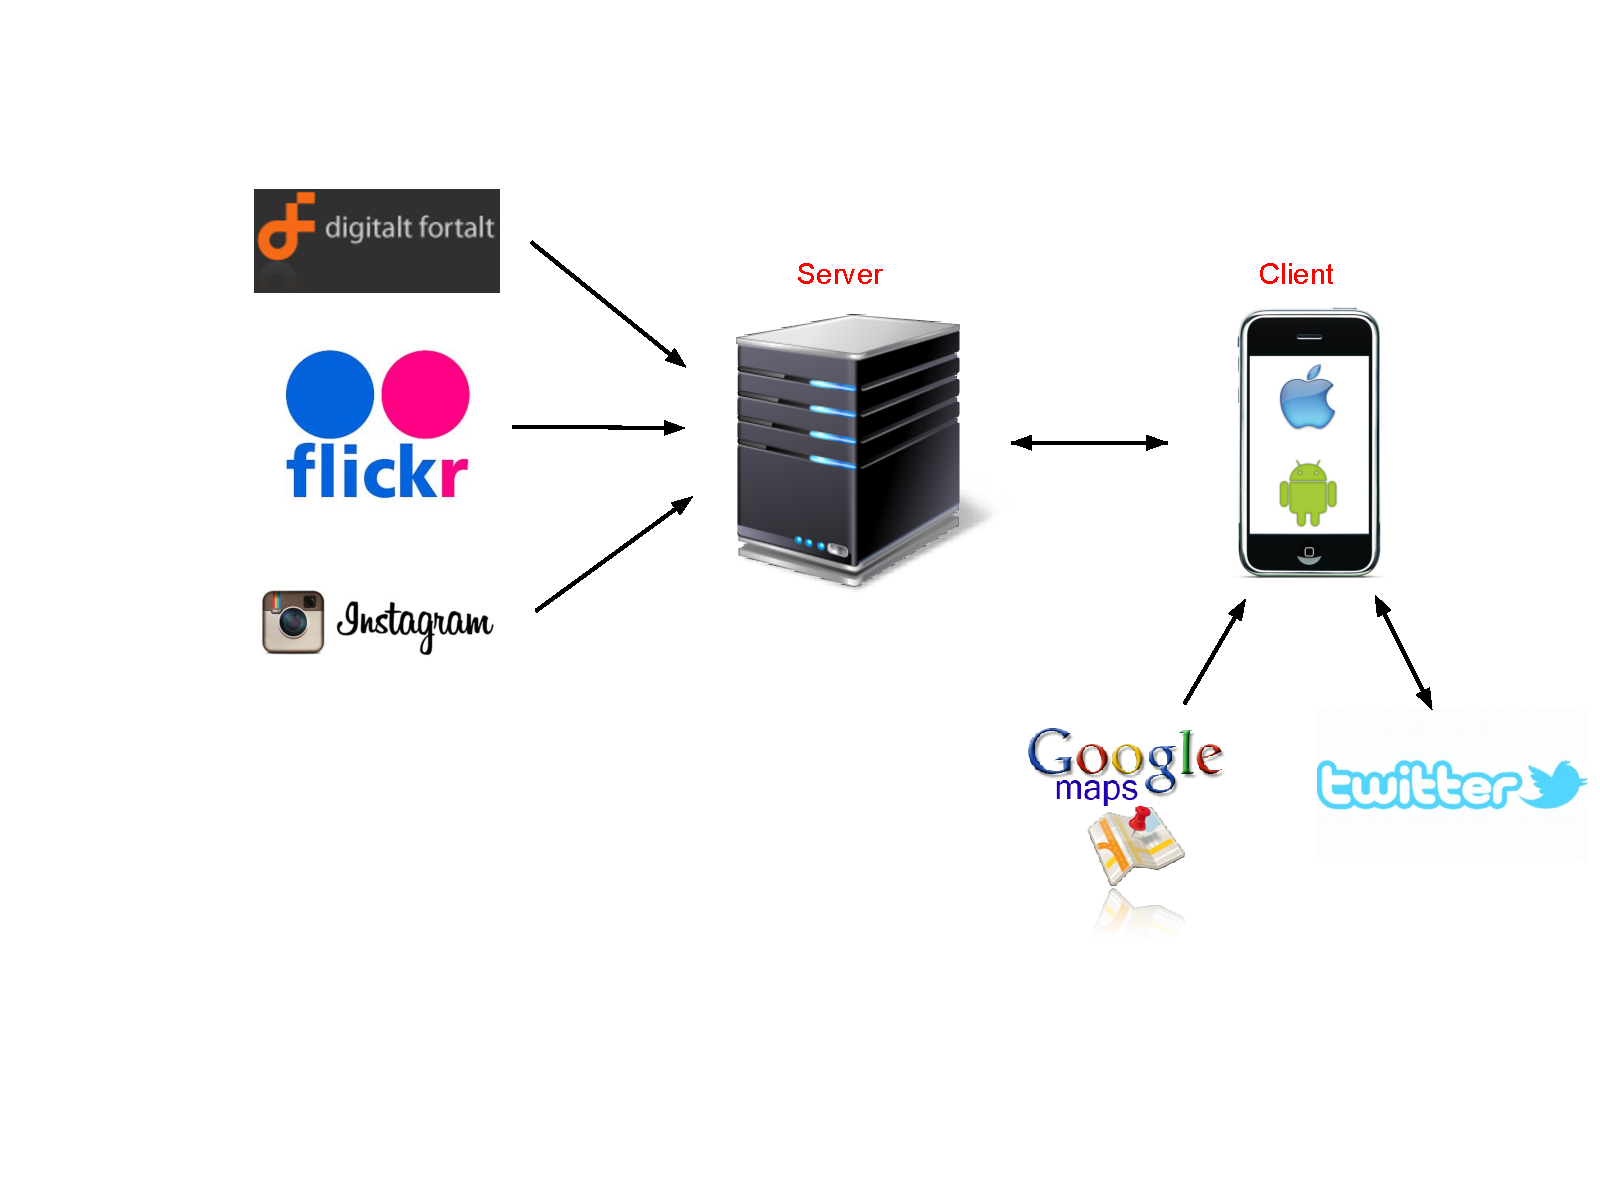
\includegraphics[scale=0.45]{ntoverview-architecture}
\caption{A simple overview of the architecture}
\end{center}
\end{figure}

\begin{itemize}
\item Browse a map and zoom in and out.
\item Load \textbf{places}.
\item Click on a place in the map and access \textbf{stories} from Digitalt Fortalt.
\item Get social media related to a place from the content providers Instagram and Twitter.
\item Go to a users exact position on a map.
\item Search for a location in the map.
\end{itemize}
	
		\subsubsection{Limitations}
There are some limitations to the system that needs to be further developed, and some that probably would require total architectural review of the project to be fixed. Our task is to continue the development of the applicaton. An overview of the features we are going to improve are discussed in the requirements-section. Flaws that arised during the development which requires a new architecture will be discussed in the conclusions-section under Recommendations.

		\subsubsection{Evaluation}
		
After the first meetings we concluded that the best way to proceed is to evaluate the existing system, to uncover potential issues and flaws.
Therefor we decided that everyone should individually do a usability test when exploring the app for the first time. Here are a short summary of all our reports:\\[3pt]

When opening the application the first major issue most of us experience is how slow the app loads, with little feedback that something is actually working in the background. Another thought that generally comes to mind is \emph{I don't understand the apps function when opening it without prior knowledge}. What happens is that you get a map with tags you could click on, making you believe the apps function is to bring it when visiting a town (not Trondheim in particular) and want to explore historical monuments and get wikipedia like facts. When clicking on tags you get to the location-specific page, and there are displayed content from instagram. Some of us found this social feature not to have very obvious intentions, it can seem like theres added social interactions to the applications just because it is popular. You would want actual and useful information about the places to be the first thing displayed and get confused when suddenly a lot of instagram photos with random people posing with the attraction appear. Our first impression is that this social part have to offer something more interesting to be relevant at this point. There is added a nice touch with a slight gradient to white i the bottom indicating that you can scroll down for more content. When the phone is turned (switched to landscape mode) there are issues however, there are no scroll function here limiting the content available and the images are cropped. Also if there is lot of text added in the instagram feed, this and hashtags disappears. The way to collect images from instagram to the application also seems to be less than optimal when sometimes completely irrelevant content are displayed. When tweeting there are no limitations on length, which causes problems when trying to post tweets over 140 characters.\\
These are some of the feedback extracted from the individal tests. 

		
	\subsection{Survey}

	\todo{Sammendrag av spørreundersøkelsen som ble gjort av Øyvind}
	
	\subsection{Desired solution}
	
	\todo{Implementere requirements i en liten tekst som forklarer hva vi ønsket å oppnå med applikasjonen}
	
	\subsection{Tools and technologies}
		\subsubsection{Titanium vs Phonegap}
		\subsubsection{Digitalt fortalt API}

	\subsection{Similar products}
		\todo{produkter med ligjnende funksjonalitet og/eller produkter med liknende formål}
